\documentclass[UTF8]{beamer}
\mode<presentation> {
	\usetheme{Boadilla}
}
\setbeamertemplate{navigation symbols}{}
\usepackage[utf8]{inputenc}
\usepackage[spanish]{babel}
\usepackage{graphicx}
\usepackage{framed}
\graphicspath{{images/}}


\title[Portada]{
	Galera Cluster \\
	\large "Un verdadero multi-master sin que se rompa a los 3 minutos"\\
}
\author{Chema Alcaraz}
\date{2 de Febrero de 2017}
\titlegraphic{
\includegraphics[width=4cm]{devops_murcia}}




\begin{document}
	
\begin{frame}
	\titlepage
\end{frame}

\title{¿Quien soy?}

\begin{frame}
	\centering
	\mbox{¿Quien soy?}	
\end{frame}


\begin{frame}
\begin{columns}
    \begin{column}{0.6\textwidth}
        \begin{itemize}
            \item \textbf{Jose Maria Alcaraz (Chema Alcaraz)}
            \item Admin. Sistemas en Ortopedia Plus
            \item Medalla de Plata en SpainSkills 2013
			\item Ganador accésit Redes V Olimpiada Regional 2012
			\item Certificado por Apple como \\'Apple Product Professional' 2011
            \item Ganador IV Olimpiada FP Regional 2010
        \end{itemize}
    \end{column}
    \begin{column}{0.40\textwidth}
        
\includegraphics[width=5cm]{images/yo}
    \end{column}
\end{columns}
	
\end{frame}


\title{¿Que es Galera Cluster?}

\begin{frame}
	\centering
	\mbox{¿Que es?}	
\end{frame}


\begin{frame}
	\frametitle{¿Que es galera?}
	\begin{framed}
		Galera Cluster es un cluster síncrono multi-master para MySQL.
	\end{framed}
	\pause
	\begin{framed}
		Consiste en dos partes, la libreria de Galera (llamada actualmente `galera-3`) y la versión extendida de MySQL con la API de WSREP (Write Set Replication)
	\end{framed}
\end{frame}


\title[¿Que ganamos?]{¿Que ganamos con Galera?}
\begin{frame}
	\centering
	\mbox{¿Que ganamos con Galera?}	
\end{frame}


\begin{frame}
	\frametitle{¿Que ganamos con Galera?}
	\begin{itemize}
		\item Replicación sincrona
		\pause
		\item Topología multi-master real
		\pause
		\item Control automático de miembros del cluster
		\pause
		\item Fácil unión de nuevos miembros
		\pause
		\item Replicación paralela a nivel de fila
		\pause
		\item No tiene latencia en los 'esclavos'
		\pause
		\item No pierdes transacciones
		\pause
		\item Escalable tanto en lectura como en escritura
		\pause
		\item Latencia hacia cliente minima
		\pause
		\item Replicacion basada en certificación
	\end{itemize}
\end{frame}


\title[Limitaciones]{Limitaciones}
\begin{frame}
	\centering
	\mbox{Limitaciones}	
\end{frame}


\begin{frame}
	\frametitle[Limitaciones]{Limitaciones}
	\begin{itemize}
		\item La replicación solo funciona con InnoDB
		\pause
		\item Los bloqueos explícitos no están soportados
		\pause
		\item Todas las tablas deben llevar PRIMARY KEY
		\pause
		\item Query log debe ir a un fichero.
		\pause
		\item Las transacciones XA no están soportadas
		\pause
		\item Tamaño de la transacción.
	\end{itemize}
\end{frame}


\title[Replicación]{Replicación}
\begin{frame}
	\centering
	\mbox{¿Como funciona la replicación basada en certificación?}	
\end{frame}


\begin{frame}
	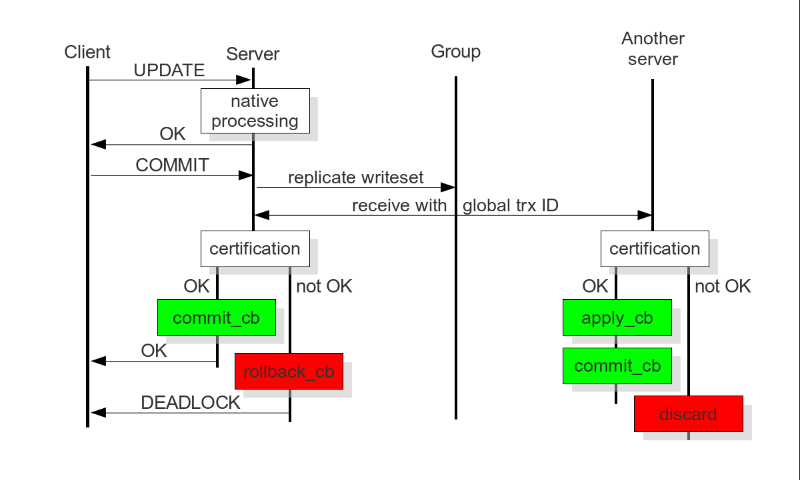
\includegraphics[width=\textwidth,height=\textheight,keepaspectratio]{images/certificationbasedreplication.png}
\end{frame}





\title[Backup]{Backup}

\begin{frame}
	\centering
	\mbox{¿Y que pasa con los backups?}	
\end{frame}

\begin{frame}
	\centering
	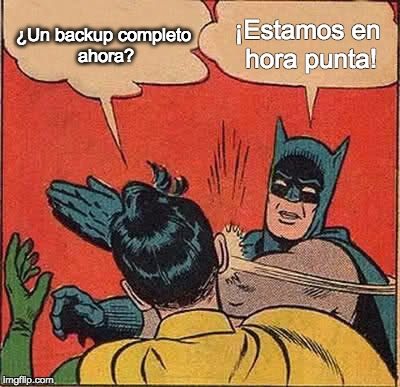
\includegraphics[width=\textwidth,height=\textheight,keepaspectratio]{necesitas_backup}
\end{frame}

\begin{frame}
	
\includegraphics[width=\textwidth,height=\textheight,keepaspectratio]{bloquear}
\end{frame}

\begin{frame}
	
\includegraphics[width=\textwidth,height=\textheight,keepaspectratio]{tenemos_xtrabackup}	
	
\end{frame}
	
	
	
	
	
	
\end{document}